\documentclass[11pt,a4paper]{article}

% ---------------------------------------------------------------------------
% Packages
% ---------------------------------------------------------------------------
\usepackage[a4paper,margin=2.5cm]{geometry}
\usepackage[utf8]{inputenc}
\usepackage[T1]{fontenc}
\usepackage{graphicx}
\usepackage{booktabs}
\usepackage{tabularx}
\usepackage{longtable}
\usepackage{array}
\usepackage{xcolor}
\usepackage{hyperref}
\usepackage{enumitem}
\usepackage{caption}
\usepackage{parskip}
\usepackage{titlesec}
\usepackage{fancyhdr}
\usepackage{amssymb}

\hypersetup{
    colorlinks=true,
    linkcolor=blue!50!black,
    urlcolor=blue!50!black,
    citecolor=blue!50!black,
    pdftitle={Hospital Patient Vital Signs Monitoring -- Technical Report},
    pdfauthor={EC8203 Mini-Project Team}
}

\pagestyle{fancy}
\fancyhf{}
\fancyhead[L]{Hospital Patient Vital Signs Monitoring}
\fancyhead[R]{EC8203 Mini-Project Report}
\fancyfoot[C]{\thepage}
\renewcommand{\headrulewidth}{0.4pt}

\titleformat{\section}{\normalfont\Large\bfseries}{\thesection}{1em}{}
\titleformat{\subsection}{\normalfont\large\bfseries}{\thesubsection}{1em}{}

% Convenience column types for wrapping table cells
\newcolumntype{L}[1]{>{\raggedright\arraybackslash}p{#1}}
\newcolumntype{C}[1]{>{\centering\arraybackslash}p{#1}}

\newcommand{\code}[1]{\texttt{\small #1}}

% ---------------------------------------------------------------------------
\title{\textbf{Hospital Patient Vital Signs Monitoring}\\[0.3em]
\large EC8203 Applied Big Data Engineering --- Mini-Project Technical Report}
\author{Akila Piumantha (Member A) \and Member B \and Layanga Rajapakshe (Member C)}
\date{30 September 2026}

% ===========================================================================
\begin{document}

\maketitle
\thispagestyle{empty}
\newpage

\tableofcontents
\newpage

% ===========================================================================
\section*{Executive summary}
\addcontentsline{toc}{section}{Executive summary}

This project builds an end-to-end \textbf{Lambda-architecture} data pipeline for a hospital ward
that answers one business question: \emph{which patients show concerning vital-sign trends right
now, and how do yesterday's lab results change the risk picture for those patients going forward?}
Bedside monitors for 20 synthetic patients stream a reading every 2 seconds into Kafka; a Spark
Structured Streaming speed layer scores each patient in near real time (a simplified NEWS2 score)
and raises alerts within seconds. Once a day, the pathology lab drops a CSV of results; an
Airflow-orchestrated batch layer validates it, recomputes the previous day's vitals from an
immutable Parquet lake, and produces a consolidated risk report showing exactly how each patient's
risk tier changed once labs were factored in. Both views meet in one PostgreSQL database and are
exposed through a FastAPI serving layer and two Grafana dashboards.

The system was built and verified as a 17-container Docker Compose stack by a team of three
(platform/ingestion/observability, the Spark speed layer, and the Airflow batch layer/serving API).
It was run continuously for soak tests exceeding 40 minutes and 9--43 simulated days, during which
every one of 13 alert rules was deliberately triggered and confirmed to resolve, and the batch
layer's daily reconciliation against the speed layer stayed below 1\% discrepancy --- direct,
measured evidence for the Lambda design decision defended in Section~\ref{sec:architecture}.

% ===========================================================================
\section{Use case and business requirements}

\textbf{Use case 2 --- Hospital Patient Vital Signs Monitoring.} A hospital ward wants continuous,
near-real-time monitoring of patient vitals from bedside sensors, correlated daily with lab test
results the pathology lab uploads once a day. We interpreted the brief as five functional
requirements and two non-functional ones.

\begin{longtable}{@{}L{1.2cm}L{6cm}L{7.5cm}@{}}
\toprule
\textbf{\#} & \textbf{Requirement} & \textbf{Where it is met} \\
\midrule
\endhead
R1 & Seconds-level awareness: a per-patient risk tier and alerts within one processing cycle of a reading &
Speed layer (Spark Structured Streaming) writing \code{patient\_status} and \code{alerts} every 5 seconds \\
R2 & Trends, not only thresholds: deterioration shows as rising heart rate, falling SpO2 or falling blood pressure over minutes, not just single bad readings &
2-minute sliding windows, per-patient trend slopes and a sustained-abnormal-window counter \\
R3 & Robust daily lab ingestion: a late, missing, corrupt or repeated file must never corrupt the data &
Airflow DAG with a file sensor, schema/row validation, quarantine, and an idempotent full-day reload \\
R4 & Labs feed back into the live view: a patient with normal vitals but an abnormal lactate is still at risk &
\code{patient\_lab\_risk}, re-read by the streaming job every micro-batch so the live tier updates within seconds of the batch layer committing \\
R5 & A trustworthy daily consolidated report: recomputed from immutable data, ranked by risk, explaining what the labs changed, reproducible for any past day &
Batch Spark job over the Parquet lake producing \code{patient\_risk\_report} plus an HTML/CSV report \\
NF1 & Runs on a single laptop &
Docker Compose, 17 containers, single-broker Kafka, single PostgreSQL instance, all with memory limits \\
NF2 & Observable and replayable &
Structured JSON logs, Prometheus metrics, 13 alert rules, and an idempotent design throughout so any day can be safely replayed \\
\bottomrule
\end{longtable}

\textbf{Simplifications stated up front} (elaborated in Section~\ref{sec:assumptions}): the patients
are synthetic and generated by a seeded simulator; one simulated day compresses to 5 real minutes;
and the risk score is a simplified adaptation of NEWS2 that omits respiration rate and consciousness
level, so it is illustrative and \textbf{not clinically validated}.

% ===========================================================================
\section{Architecture decision: Lambda, not Kappa}
\label{sec:architecture}

We chose a \textbf{Lambda architecture}. The business question has two halves with genuinely
different latency, replay and consistency requirements, and Lambda lets each half use the
processing model that fits it, merging the results in one serving store.

\begin{longtable}{@{}L{5.5cm}L{9.2cm}@{}}
\toprule
\textbf{Requirement} & \textbf{How Lambda meets it} \\
\midrule
\endhead
Alerts within seconds & Speed layer: Spark Structured Streaming, 5-second micro-batches, event-time windows \\
Labs arrive as one daily file, sometimes late or corrected & Batch layer: an Airflow sensor, then validate then load; there is no need to force a file-based source through a log \\
The daily report must be correct, not approximate & The batch job recomputes the whole day from the immutable Parquet lake, including late data the speed layer's watermark dropped \\
Replay or backfill any past day & Re-run the batch job for \code{sim\_day = N}, independent of Kafka's 24-hour retention \\
One scoring logic across both layers & \code{common/scoring.py} is imported by both the streaming job and the batch job, so the two views cannot silently diverge in their rules \\
\bottomrule
\end{longtable}

\textbf{Rejected alternative: Kappa.} A single streaming codebase would process both vitals and
labs (labs published to a compacted Kafka topic) and ``reprocess'' history by replaying the log. We
rejected this for three reasons. First, reprocessing a day still needs the full log somewhere ---
either very long Kafka retention or a lake to replay from, which is exactly the batch storage Lambda
already has, so Kappa does not remove that cost, it only hides it. Second, the daily report's natural
semantics are ``recompute and overwrite the partition for day N'', which is simpler and safer to
reason about as an idempotent batch job than as a long-running stateful streaming job with the same
guarantee. Third, the lab file is batch by nature (one delivery a day, occasionally late or
corrected), and the assignment's mandated orchestrator, Airflow, would have nothing meaningful to
orchestrate under Kappa.

\textbf{The cost of Lambda, paid honestly.} Two code paths can drift apart. We mitigate this with the
shared scoring module above, and --- rather than assume the two views agree --- we \emph{measure}
the disagreement every simulated day: the batch layer publishes \code{speed\_batch\_discrepancy\_ratio},
comparing its exact per-window aggregates against the speed layer's windowed ones. A non-zero ratio
is expected, because the speed layer deliberately trades completeness for latency (readings later
than its 1-minute watermark are excluded from windows, though they remain in the lake). Over a
43-simulated-day soak run this ratio averaged \textbf{0.54\%} (min 0.13\%, max 0.99\%) --- an order
of magnitude below the 10\% alert threshold --- with zero windows the speed layer failed to produce
and a mean heart-rate difference of at most 0.034~bpm per window. This is the strongest evidence for
the architecture decision: the trade-off Lambda makes explicit is small, quantified, and continuously
monitored rather than assumed away.

\textbf{Ingestion and replay.} The Kafka topic \code{vitals.raw} has 3 partitions keyed by
\code{patient\_id}, guaranteeing per-patient ordering (required for trend slopes) with enough
parallelism for 20 patients. Retention is a short 24 hours because Kafka is a transport, not the
system of record --- replaying history reads the Parquet lake, which is exactly-once per reading and
retained indefinitely, rather than the at-least-once topic. Kafka's own offsets are used only for a
narrower kind of replay: resuming the speed layer from its checkpoint after a restart, which its
short retention window is sized for.

\textbf{Serving and consistency.} The speed and batch views meet in one PostgreSQL database at two
points with different consistency guarantees. Lab risk reaches the live view \emph{eventually
consistently}: the streaming job re-reads the newest \code{patient\_lab\_risk} row every micro-batch,
so a patient's tier reflects yesterday's labs within about 5 seconds of the batch layer committing,
and a quarantined lab file leaves the previous lab risk in force rather than dropping it to zero. The
daily report is \emph{strongly consistent} by construction: it is computed from the immutable lake,
not the speed tables, so late data and duplicates are handled correctly and replaying a day
reproduces an identical report. The API exposes the freshness of each side (data age, latest report
day, latest lab day) so a reader can see how current each part of the answer is.

% ===========================================================================
\section{Architecture diagram}

Figure~\ref{fig:architecture} shows data flowing through the four layers the assignment asks for:
ingestion, processing, storage and serving. The one dashed arrow is the detail that makes the
business question answerable: the speed layer re-reads \code{patient\_lab\_risk} every micro-batch,
so a lab result the batch layer just computed changes a patient's live risk tier within seconds, not
the next day.

\begin{figure}[h]
\centering
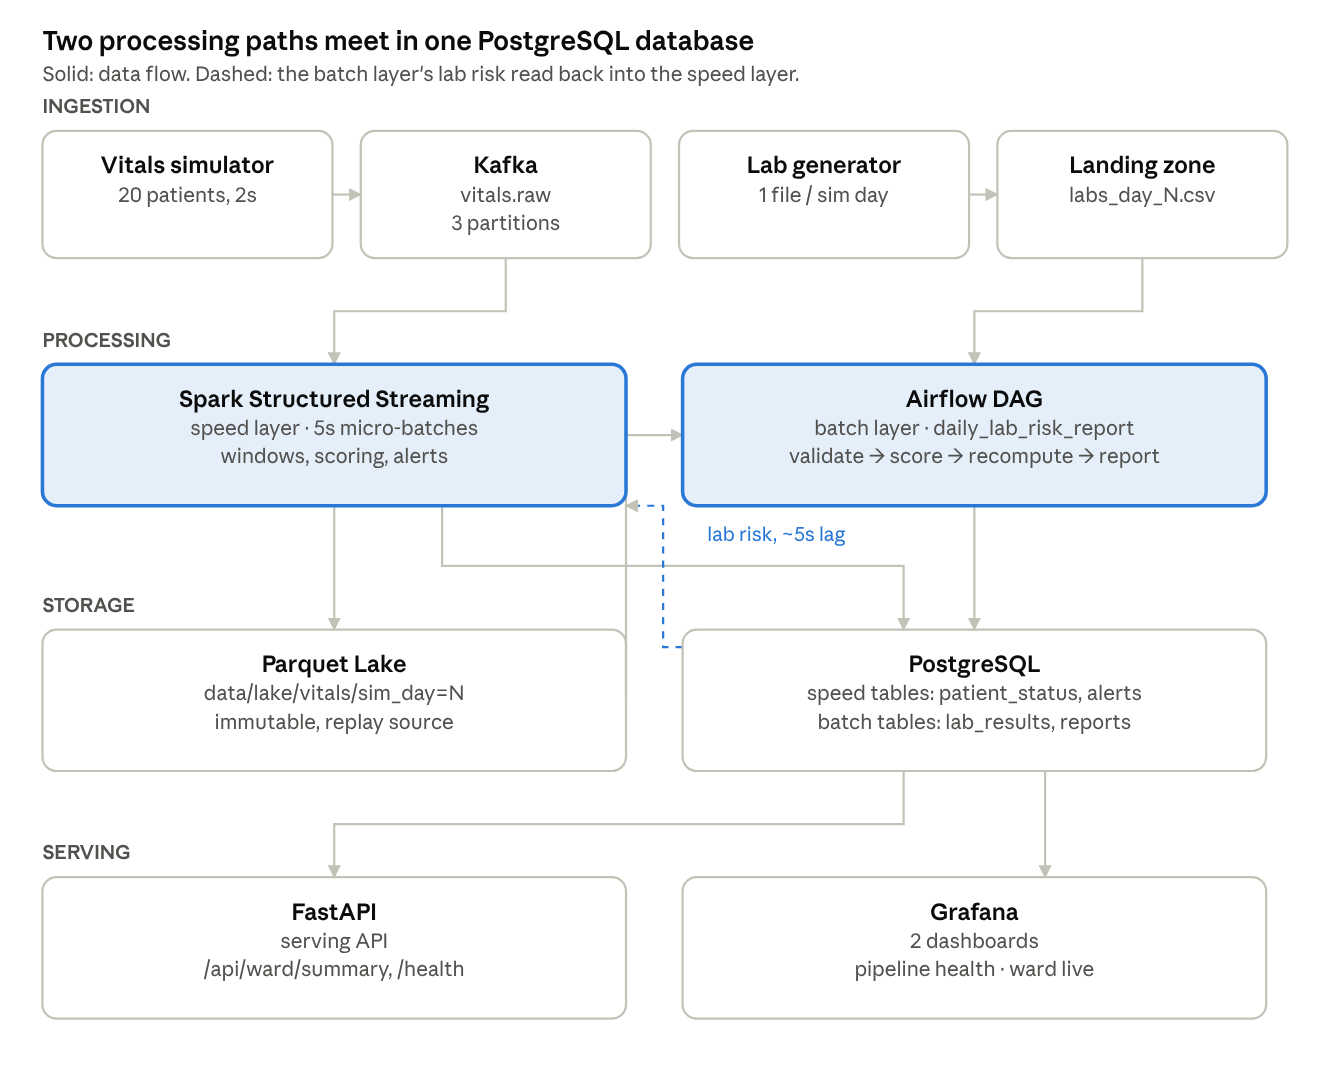
\includegraphics[width=\textwidth]{figures/architecture-diagram.png}
\caption{System architecture: ingestion, processing, storage and serving layers, with the lab-risk
feedback loop from the batch layer back into the speed layer.}
\label{fig:architecture}
\end{figure}

% ===========================================================================
\section{Technology stack}

Every choice below is justified against this use case's constraints, not general popularity.

\begin{longtable}{@{}L{2.6cm}L{4.2cm}L{7.9cm}@{}}
\toprule
\textbf{Layer} & \textbf{Choice} & \textbf{Why this use case needs it} \\
\midrule
\endhead
Ingestion & Kafka (KRaft, 1 broker), topic \code{vitals.raw} with 3 partitions keyed by \code{patient\_id}, plus \code{vitals.dlq} &
Per-patient ordering is a correctness requirement for trend slopes, not a nice-to-have. A log decouples 20 independent bedside monitors from a speed layer that may be temporarily down and gives it something to resume from after a restart. \\
Stream processing & Spark Structured Streaming &
The business question needs event-time windows and watermarks over deliberately out-of-order sensor data, plus a stream-static join against daily lab risk that must pick up new rows without a restart --- both native to Structured Streaming. Apache Storm was rejected: it would need hand-rolled state management to reach the same windowing and join semantics this project gets natively. \\
Orchestration & Apache Airflow, LocalExecutor &
The lab side is a genuine multi-step batch dependency chain (wait for file, validate, load, score, recompute, report, health-check, archive) with retries and a visible run history --- exactly Airflow's job. The DAG is the entire batch half of the Lambda architecture, not a token integration. \\
Storage / serving & PostgreSQL for speed and batch tables; Parquet on a local volume (standing in for S3/HDFS) for the lake &
Postgres: the write pattern is small, frequent upserts (about 20 patient rows plus about 100 window rows every 5 seconds) with ad-hoc SQL joins across speed and batch tables --- a poor fit for Cassandra's append-oriented, join-averse model at this scale. Parquet: the lake must be cheaply re-scannable by simulated day for the batch recompute and for replay; a columnar, partition-pruned format is the natural fit, and the brief explicitly allows a file system with Parquet in place of a database for this role. \\
Serving API & FastAPI &
Read-only endpoints over both layers' tables, OpenAPI documentation generated from the response models so the docs cannot drift from the code, and a natural home for \code{/health} and \code{/metrics}. \\
Observability & Prometheus, Alertmanager, Grafana, structured JSON logs &
Every component here is a different language and runtime (Python, JVM, Airflow); Prometheus's pull model plus one shared metric-naming contract let a single dashboard and a single alert-rule set cover all of them without any component needing to know about the others. \\
Packaging & Docker Compose, one file per layer joined by \code{include:} &
Three team members each own a Compose fragment (\code{compose/spark.yml}, \code{compose/airflow.yml}, \code{compose/api.yml}) without ever touching the same file --- a direct, practical answer to three people needing to work in parallel, not a generic default. \\
\bottomrule
\end{longtable}

% ===========================================================================
\section{Data ingestion implementation}

\textbf{Two simulated sources}, both plain Python processes with no framework, so every number in
the report can be traced back to a line of generator code.

\emph{Vitals stream} (\code{simulators/vitals\_producer.py}): 20 synthetic patients, each with a
physiological baseline (heart rate, SpO2, systolic/diastolic blood pressure, temperature) drawn once
from a seeded cohort and perturbed every 2 seconds by mean-reverting noise. Four scripted patients
carry a deterioration episode (sepsis-like or respiratory) that ramps, holds and recovers; two
further ``occult'' patients keep normal vitals throughout but their labs turn abnormal from a fixed
simulated day on. This scripted, known-in-advance ground truth (\code{data/ground\_truth/episodes.json})
is what makes it possible to check that alerts, the lab-risk feedback loop and the daily report catch
the right patients, rather than merely running without crashing.

\emph{Lab file} (\code{simulators/lab\_generator.py}): one CSV per simulated day
(\code{labs\_day\_N.csv}), correlated with the same scripted story --- abnormal lactate, white cell
count and CRP while a sepsis episode is active; abnormal creatinine, potassium or glucose for chronic
conditions; abnormal results for the occult patients from their trigger day. Files are written to a
temporary path and atomically renamed into place, so a consumer can never observe a half-written
file.

\textbf{Robustness and fault injection.} The Kafka producer is idempotent (\code{acks=all}, unlimited
retries) so a broker-side retry cannot itself create the duplicates the pipeline is built to
tolerate. A configurable fault injector (\code{FAULT\_PROFILE=off|low|chaos}) deliberately introduces
null vitals, physiologically impossible values, duplicate event IDs, events held back 20--90 seconds
past their timestamp, and short sensor dropouts --- not as noise, but so that validation,
deduplication, watermark handling and alerting have something real to prove themselves against
(Section~\ref{sec:results} shows the results of exercising this). Both sources derive \code{sim\_day}
from one shared, race-free simulated clock (a single epoch agreed by whichever process starts first,
verified under concurrent start-up in unit tests), and every random choice is seeded, so a given seed
always reproduces the same cohort, episodes and lab values.

% ===========================================================================
\section{Processing layer}

\subsection{Speed layer (Spark Structured Streaming)}

Two streaming queries read \code{vitals.raw}, each with its own checkpoint so they recover
independently:

\begin{enumerate}[label=\arabic*.]
\item \textbf{\code{vitals\_readings}} (5-second trigger): parses each record against an explicit
schema, marks (never silently drops) the first validation rule it fails as a \code{rejection\_reason},
joins against the \code{patients} dimension and the newest \code{patient\_lab\_risk} row (a
stream-static join re-planned every micro-batch, which is how a lab result reaches the live view
without restarting the job), computes MAP, pulse pressure, the NEWS sub-scores and the total risk
tier, then de-duplicates on \code{event\_id} within a watermark. Valid rows are written to the
Parquet lake and to \code{patient\_status}; invalid rows go to \code{vitals.dlq} and \code{dlq\_events}.
\item \textbf{\code{vitals\_windows}} (5-second trigger, update mode): the valid stream is
watermarked at 1 minute, de-duplicated again, and aggregated into 2-minute windows sliding every 30
seconds (scaled down from the plan's 5-minute reference window to match the compressed simulated
clock). Trend slopes and a sustained-abnormal-window counter are computed in the driver over the
small, bounded set of recent windows per patient.
\end{enumerate}

The risk score is a simplified NEWS2 adaptation (sub-scores for heart rate, SpO2, systolic blood
pressure and temperature) plus lab points capped at 4, giving four tiers: LOW, MEDIUM, HIGH,
CRITICAL. It is shared with the batch layer through one module, \code{common/scoring.py}, so the two
layers cannot silently apply different rules. Alerts (reason codes such as \code{TOTAL\_SCORE\_HIGH},
\code{SUSTAINED\_ABNORMAL}, \code{WORSENING\_TREND}) follow an open-to-resolved lifecycle with
deterministic IDs, so replaying a micro-batch re-derives the same alerts rather than duplicating them.

\subsection{Batch layer (Airflow)}

The DAG \code{daily\_lab\_risk\_report} runs once per simulated day: a file sensor waits for the
day's lab CSV, \code{validate\_lab\_file} checks schema, types, reference ranges and duplicate or
unknown patients (quarantining bad rows or the whole file rather than failing the run),
\code{load\_lab\_results} replaces that day's rows in one transaction, \code{compute\_lab\_risk}
derives lab points into \code{patient\_lab\_risk} (immediately visible to the speed layer above),
\code{batch\_vitals\_job} is a separate Spark job in local mode that recomputes the previous day's
vitals from the immutable lake and reconciles them against the speed layer's own windows,
\code{build\_risk\_report} produces \code{patient\_risk\_report} plus an HTML/CSV report ranked by
risk with an explicit before-labs/after-labs comparison, and a health check and archive step close
out the run. Every task writes a row to \code{pipeline\_run\_log}, and every failure increments a
Prometheus counter and triggers the matching alert (Section~\ref{sec:observability}).

Both queries and the DAG are idempotent by design: a day can be replayed (\code{make replay-day
DAY=N}) and produces byte-identical downstream rows, verified in the test suite and confirmed live by
killing and restarting both the streaming job and the Airflow scheduler mid-run
(Section~\ref{sec:results}).

% ===========================================================================
\section{Storage and serving layer}

\begin{longtable}{@{}L{2.3cm}L{4.8cm}L{3.2cm}L{4.4cm}@{}}
\toprule
\textbf{Store} & \textbf{Content} & \textbf{Key / layout} & \textbf{Why} \\
\midrule
\endhead
Parquet lake & Every valid reading plus event time, MAP, pulse pressure, NEWS score and Kafka coordinates &
\code{data/lake/vitals/sim\_day=N/part-<checkpoint>-b<batch>-NNN.parquet} &
Immutable master dataset for the batch layer; columnar and partition-pruned by day; file names include the checkpoint and micro-batch id so a replay overwrites only its own files, never duplicating or clobbering older ones \\
\code{vitals\_window} & Per patient, per 2-minute window: average/min/max of five vitals, count, window NEWS, trend slopes &
PK \code{(patient\_id, window\_start)} &
Upsert target of the update-mode streaming query; feeds the ward dashboard's time-series charts \\
\code{patient\_status} & One row per patient: latest vitals, scores, lab points, risk tier, trend flag &
PK \code{patient\_id} &
The ``right now'' ward view in O(patients) time; a guarded upsert ensures \code{last\_reading\_at} never moves backwards \\
\code{alerts} & Alert open/resolved lifecycle &
PK \code{alert\_id} (deterministic UUID), unique open alert per patient and reason &
Replay-safe: re-processing a batch cannot open a duplicate alert \\
\code{lab\_results}, \code{patient\_lab\_risk}, \code{patient\_risk\_report}, \code{batch\_vitals\_daily}, \code{speed\_batch\_reconciliation} & Daily batch outputs &
Keyed by simulated day and patient &
Written by the Airflow DAG; \code{patient\_risk\_report} is what the consolidated daily report is rendered from \\
\bottomrule
\end{longtable}

PostgreSQL was chosen over Cassandra because the write pattern here is small, frequent upserts with
ad-hoc SQL joins between the speed and batch tables --- exactly what Postgres is good at and
Cassandra is not. The \textbf{serving layer} is a FastAPI application with thirteen read-only
endpoints in five groups: ward (\code{/api/ward/summary} merges both layers in one response),
patients (paginated, sorted by risk, with a detail view joining live status to the newest lab risk),
alerts, reports (JSON and rendered HTML for any past day), and operations (\code{/health} returns a
503 when the newest reading is older than 60 seconds, \code{/metrics} exposes request latency, data
freshness, patients per tier and open alerts per severity). The API holds a small pool of read-only,
time-limited transactions, so a slow query cannot pin a connection, and a database outage returns a
clean 503 instead of a stack trace. Two Grafana dashboards (Pipeline Health over Prometheus, Ward
Live Monitoring over PostgreSQL) are provisioned as code and require no manual setup after
\code{docker compose up}.

% ===========================================================================
\section{Observability design}
\label{sec:observability}

\textbf{What is measured and why:}

\begin{longtable}{@{}L{4.3cm}L{4.8cm}L{5.4cm}@{}}
\toprule
\textbf{Signal} & \textbf{Instrument} & \textbf{Question it answers} \\
\midrule
\endhead
Is data still arriving? & \code{simulator\_last\_emit\_timestamp\_seconds}, Kafka topic offsets, \code{pipeline\_last\_event\_age\_seconds} & Has the pipeline gone silent? \\
Is the speed layer keeping up? & \code{kafka\_consumergroup\_lag}, \code{spark\_batch\_duration\_seconds} & Is processing falling behind ingestion? \\
Is data quality holding? & \code{vitals\_valid\_total}, \code{vitals\_dlq\_total\{reason\}} & What fraction of readings are rejected, and why? \\
Is the batch layer on schedule? & \code{airflow\_dag\_last\_success\_timestamp\{dag\_id\}}, \code{lab\_file\_missing\_total} & Did today's report actually get produced? \\
Do the two Lambda views agree? & \code{speed\_batch\_discrepancy\_ratio} & Is the architecture's core trade-off staying small? \\
Is the ward-facing surface healthy? & \code{api\_request\_duration\_seconds}, \code{/health} & Does the API respond, and is its data fresh? \\
\bottomrule
\end{longtable}

\textbf{Structured logging.} Every service, Python or JVM, writes one JSON object per stdout line
through a shared formatter: \code{\{ts, level, service, stage, event, run\_id, ...\}}, where
\code{stage} is one of ingestion, processing, storage, serving, orchestration or observability. This
lets a single \code{docker compose logs | grep} isolate one pipeline stage across every container
with no service-specific knowledge, and every line carries a correlation id for one container's
lifetime.

\textbf{Thirteen alert rules}, written as Prometheus rules-as-code and unit-tested against synthetic
time series with \code{promtool} before the components they depend on even existed --- several rules
reference metrics owned by the other two team members
(\code{kafka\_consumergroup\_lag\{consumergroup="spark-speed-layer"\}}, \code{airflow\_dag\_last\_success\_timestamp}),
and having them verified in advance turned integration into confirming names rather than debugging
alert logic under time pressure.

\begin{longtable}{@{}L{4.5cm}L{10cm}@{}}
\toprule
\textbf{Alert} & \textbf{Trigger condition} \\
\midrule
\endhead
\code{NoVitalsData} & No Kafka offset growth on \code{vitals.raw} for 45 seconds \\
\code{SimulatorDown} / \code{StreamingQueryStopped} / \code{ApiDown} / \code{ScrapeTargetDown} & The corresponding component stops answering its metrics endpoint \\
\code{ProducerDeliveryErrors} & Any sustained Kafka delivery failure rate \\
\code{DlqRateHigh} & More than 5\% of readings rejected by validation over 2 minutes \\
\code{ConsumerLagHigh} & The speed layer's consumer group falls more than 500 messages behind \\
\code{PipelineDataStale} & Newest processed reading older than 60 seconds \\
\code{SparkBatchSlow} & Micro-batches sustained above 10 seconds against a 5--10 second trigger \\
\code{LabFileMissing} & The daily file sensor times out \\
\code{DagFailed} & No successful DAG run in over 11 minutes (two missed simulated days) \\
\code{SpeedBatchDiscrepancy} & Speed-versus-batch reconciliation exceeds 10\% \\
\bottomrule
\end{longtable}

Alerts route through Alertmanager to a small webhook that logs every firing and resolved transition
as a structured line and appends it to a durable file (\code{data/alerts/alerts.jsonl}), independent
of Prometheus's own retention --- the evidence trail behind every claim in Section~\ref{sec:results}.
A deliberate design choice: \code{NoVitalsData} uses an \code{absent()} guard because ``no data at
all'' is itself the failure, but \code{DagFailed} does not, because before the very first DAG success
there is no time series to be absent, and guarding it would open a false alert on every fresh
\code{docker compose up} while Airflow initialises.

% ===========================================================================
\section{Results}
\label{sec:results}

All figures below come from the live, full 17-container stack, not a mock-up.

\textbf{Pipeline health dashboard}, captured across a 40-minute window that deliberately included
every fault demonstration in this report (a Spark restart, a chaos-level fault injection, and an
11-minute Airflow outage): the Kafka throughput dip and recovery, the DLQ spike during
\code{DlqRateHigh}, the consumer-lag spike and drain, the micro-batch slowdown during resource
contention, and the ``seconds since last DAG success'' sawtooth climbing to its \code{DagFailed} peak
before resetting on recovery. By the end of the window every metric is back at baseline and 0 alerts
are firing.

\begin{figure}[h]
\centering
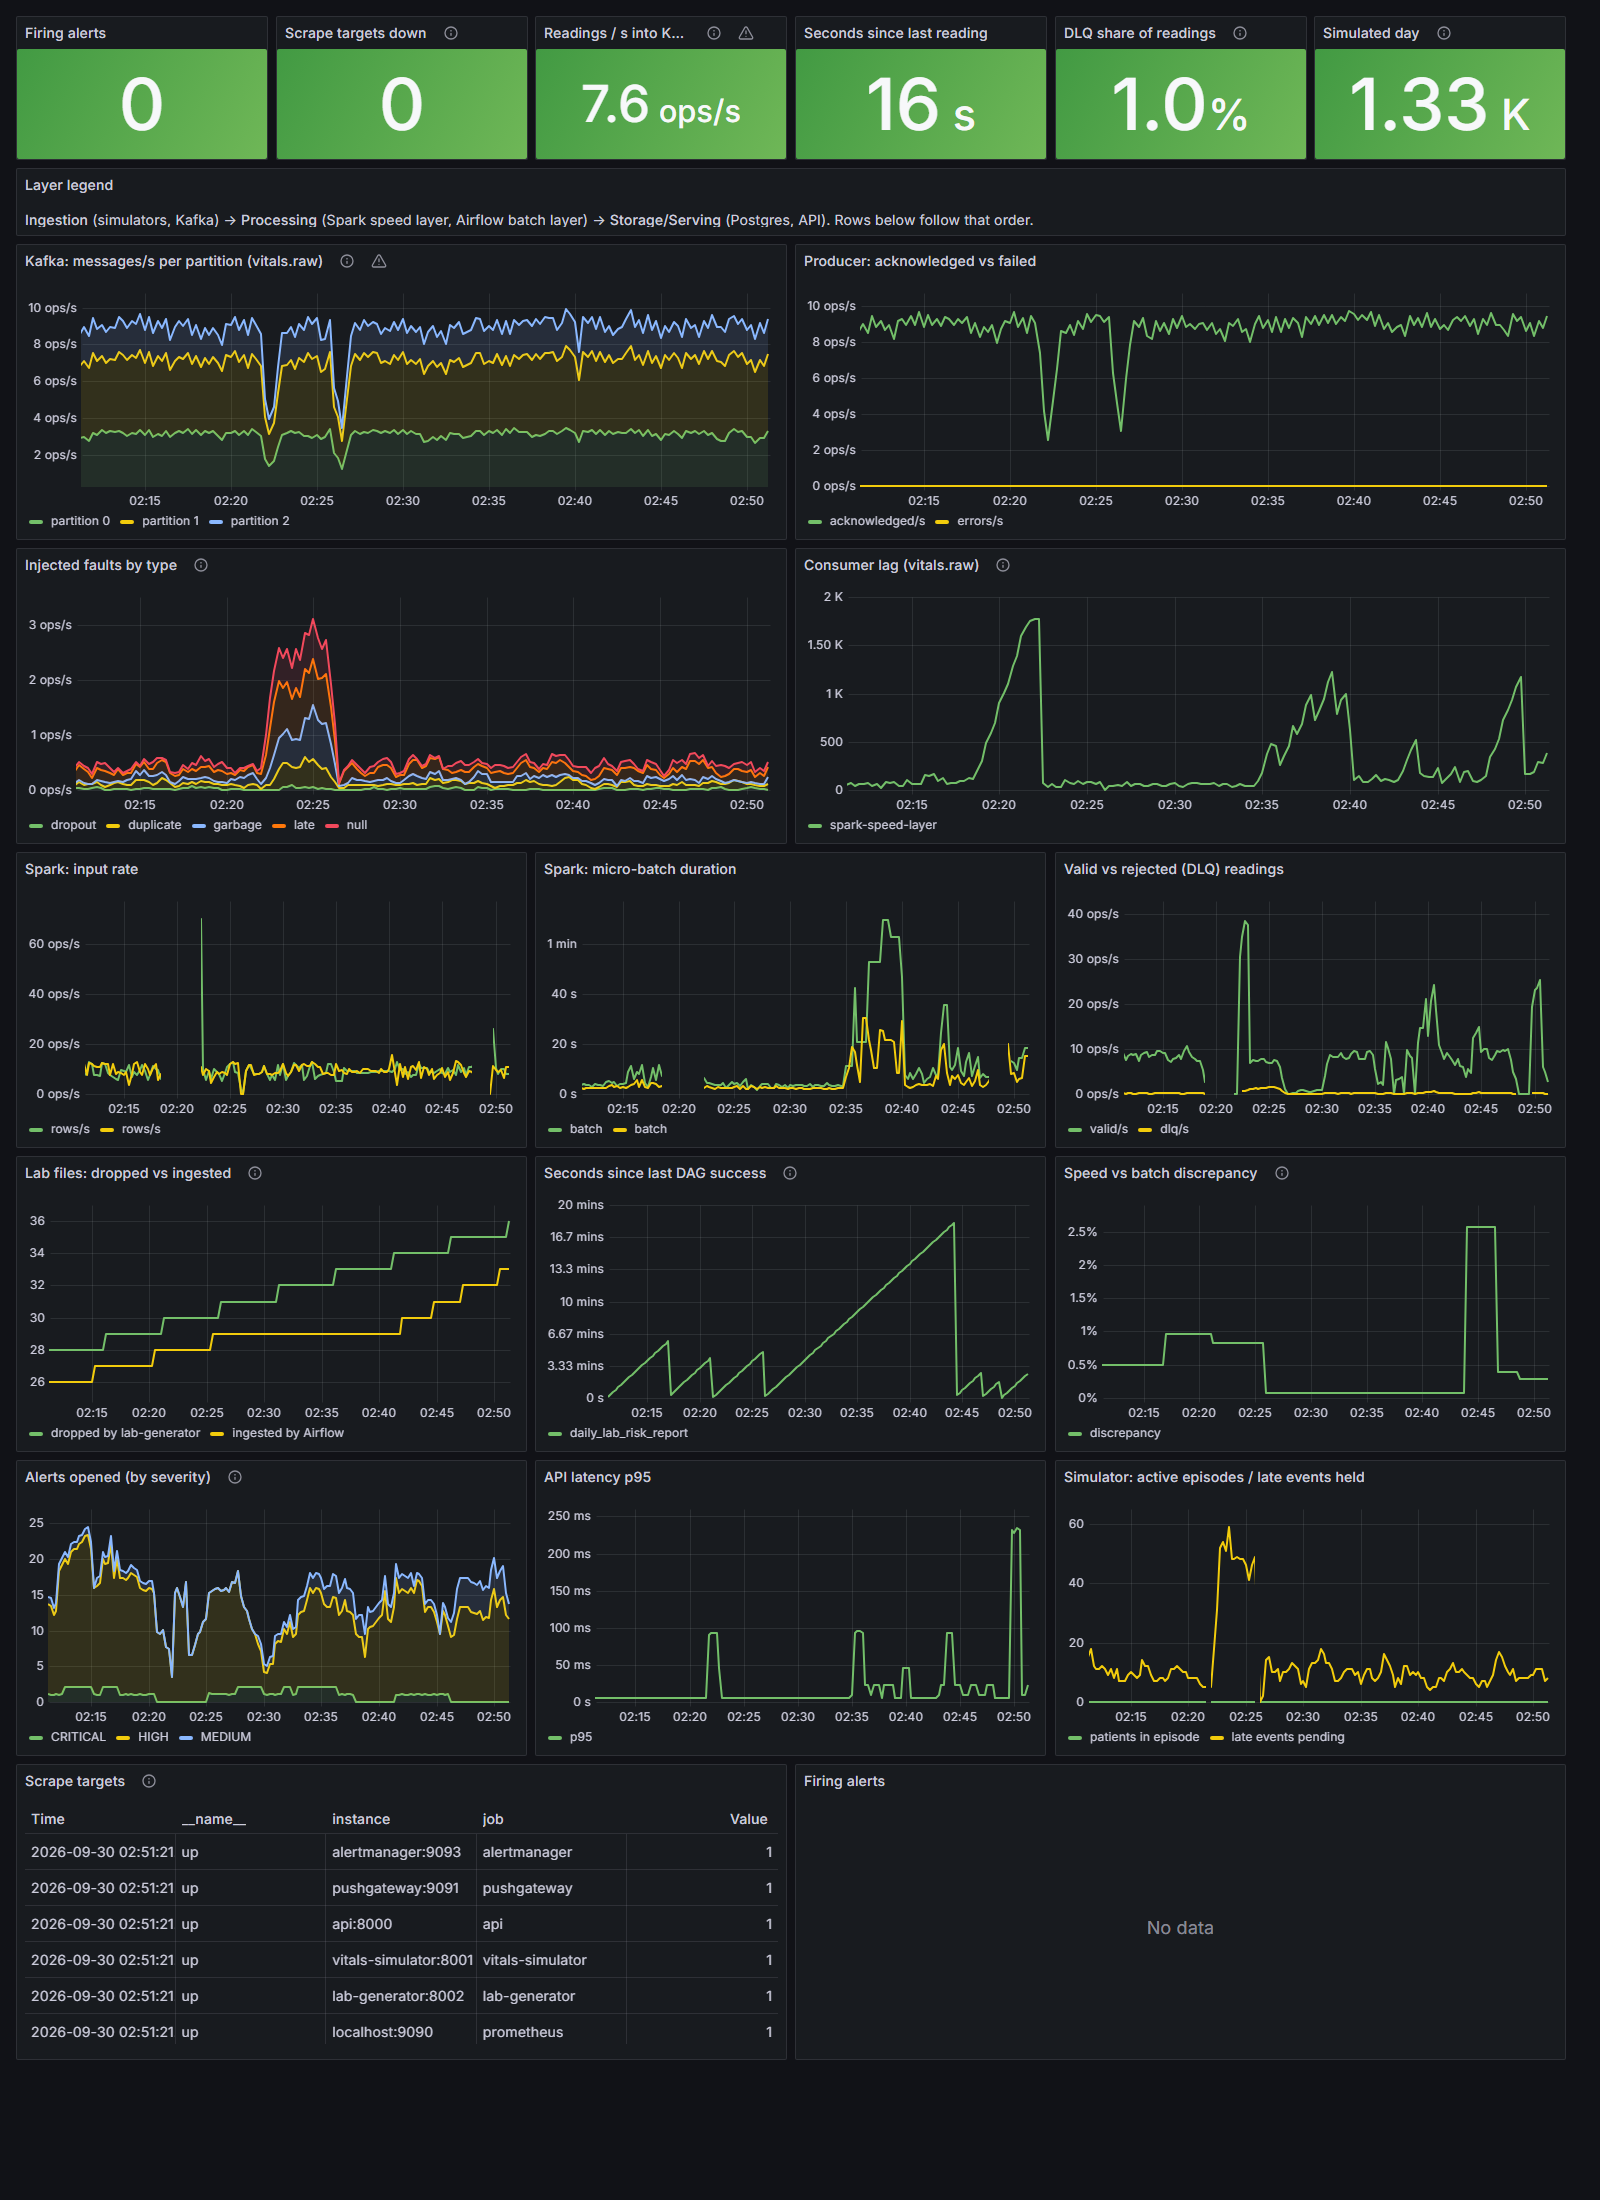
\includegraphics[width=\textwidth]{figures/fig-pipeline-health.png}
\caption{Pipeline health dashboard over the full demonstration window.}
\end{figure}

\textbf{Ward live monitoring dashboard}: current risk tiers across the 20-patient cohort, open
alerts, per-patient vital-sign trends, and, critically for this use case, the daily risk report table
showing patients whose tier changed once labs were applied (P005 and P012 rising to MEDIUM on
abnormal lab points, P018 dropping back to LOW).

\begin{figure}[h]
\centering
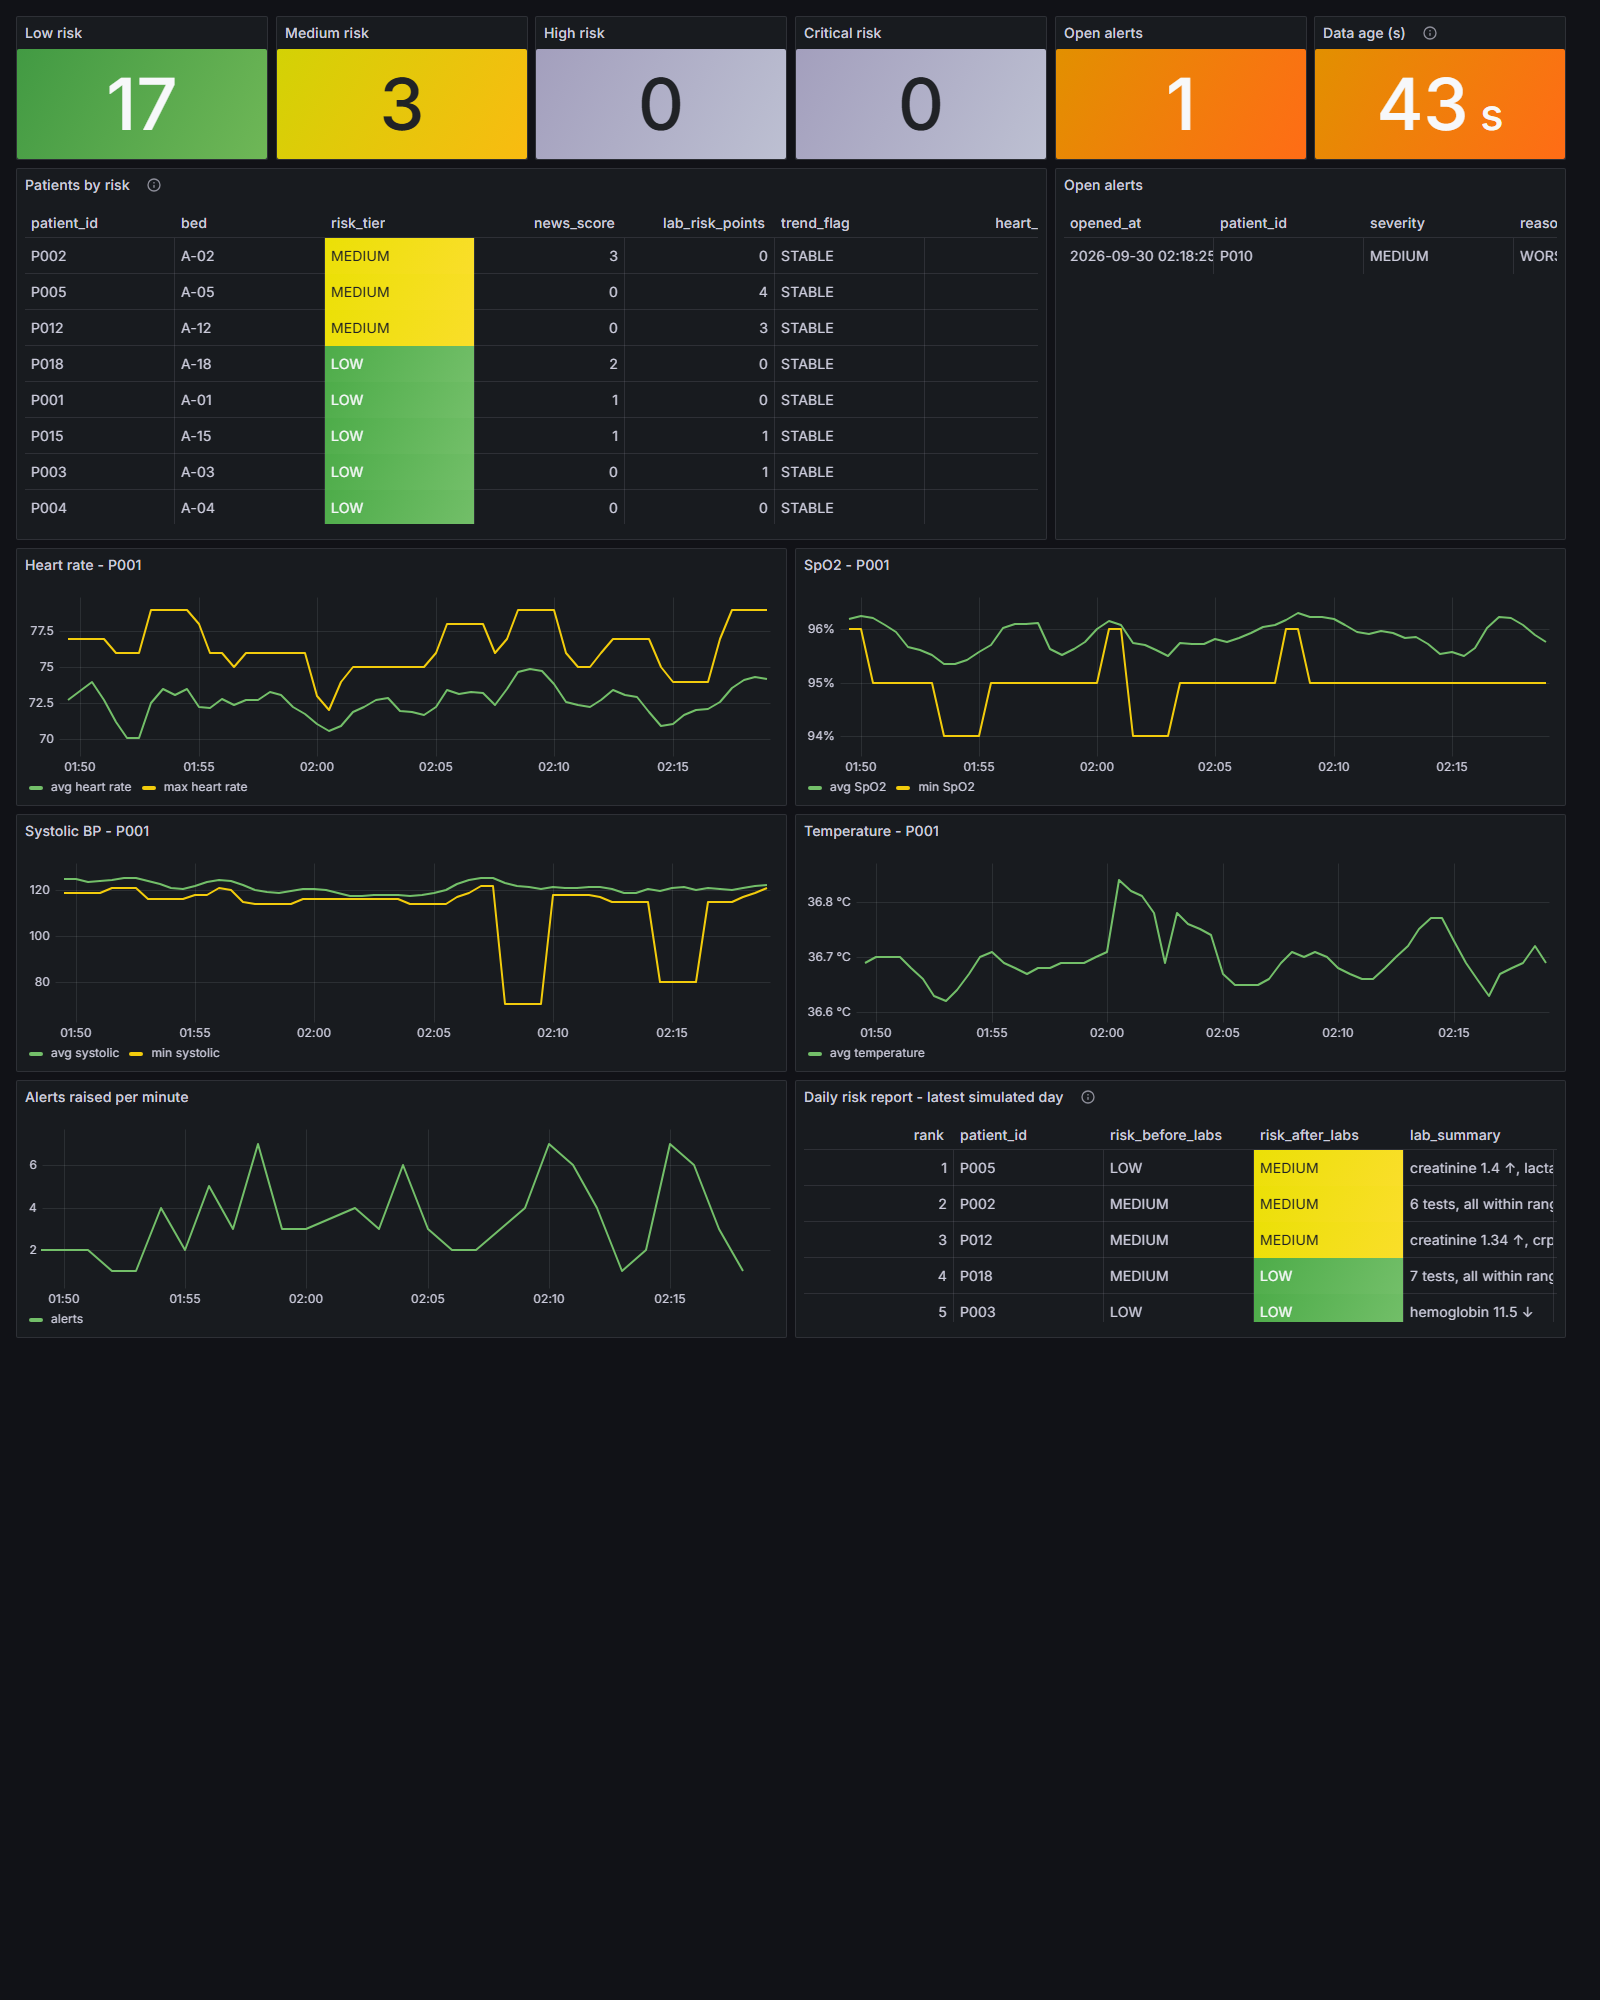
\includegraphics[width=\textwidth]{figures/fig-ward-live.png}
\caption{Ward live monitoring: risk tiers, alerts, vitals and the lab-driven daily report.}
\end{figure}

\textbf{Sample consolidated daily report} (rendered HTML, one simulated day): patients ranked by risk
after labs, with an explicit risk-before-labs versus risk-after-labs comparison, the artefact that
most directly answers the assignment's business question.

\begin{figure}[h]
\centering
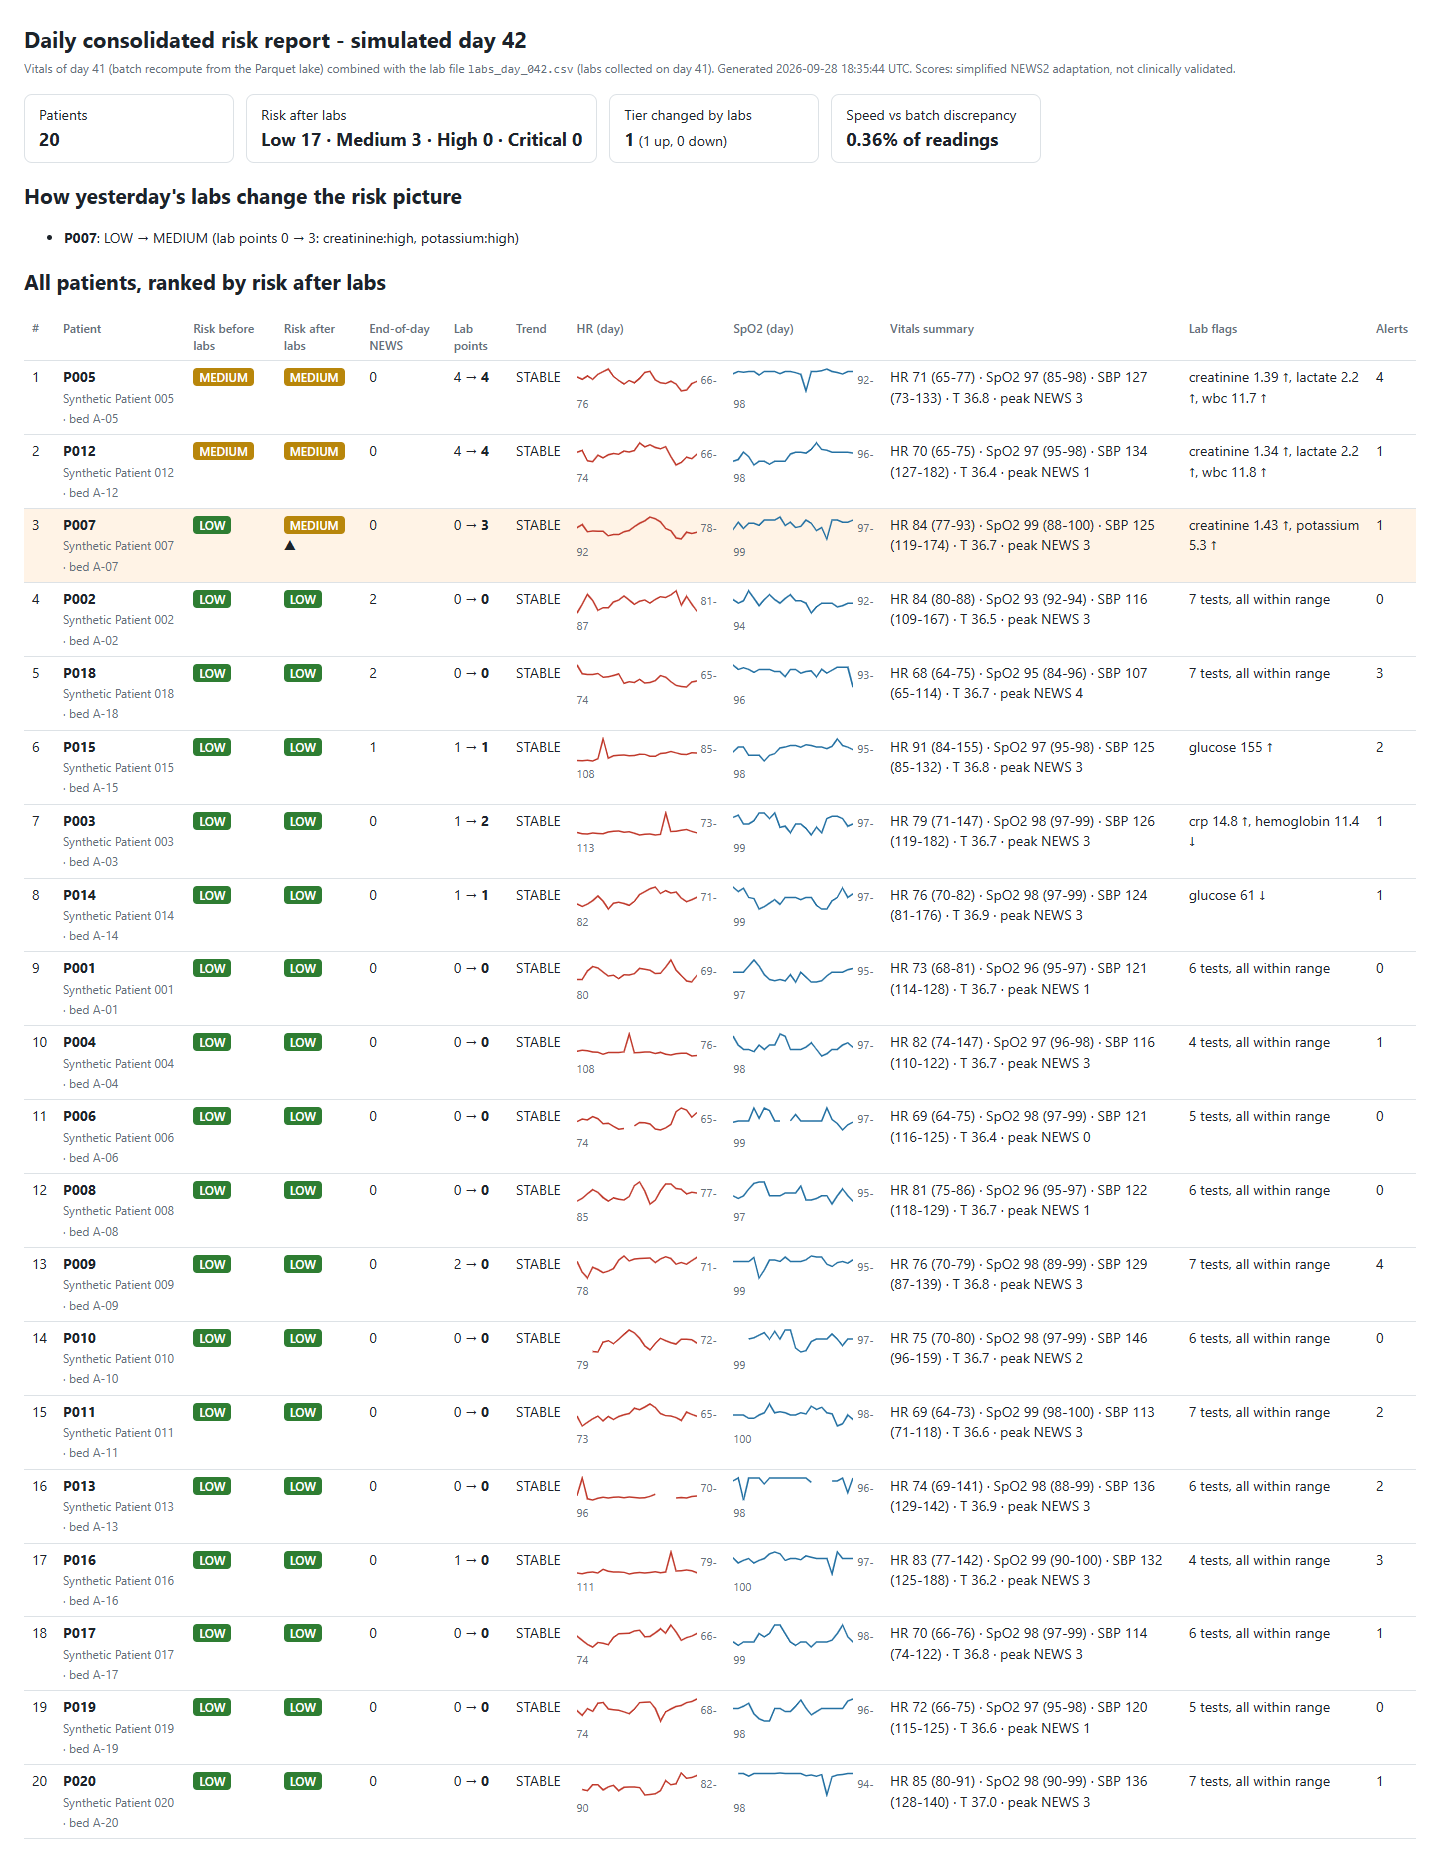
\includegraphics[width=\textwidth]{figures/fig-daily-report.png}
\caption{Sample daily consolidated risk report.}
\end{figure}

\textbf{Sample API output} (\code{/api/ward/summary}), combining live speed-layer state with the
latest batch-layer report and reconciliation in one response:

\begin{figure}[h]
\centering
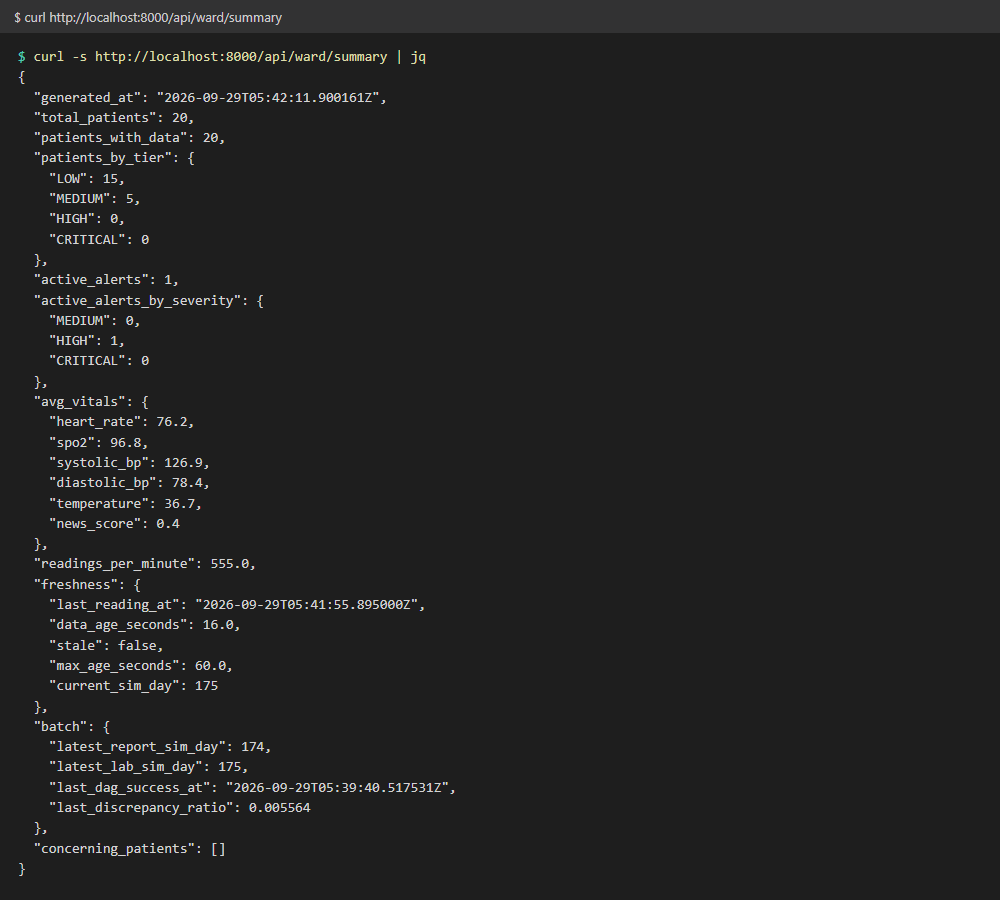
\includegraphics[width=0.8\textwidth]{figures/fig-api-sample.png}
\caption{Sample \code{/api/ward/summary} response.}
\end{figure}

\textbf{Measured soak-run results.}

\begin{longtable}{@{}L{4.7cm}L{4.5cm}L{5cm}@{}}
\toprule
\textbf{Metric} & \textbf{Platform layer alone (2026-09-25)} & \textbf{Full stack, demos included (2026-09-29/30)} \\
\midrule
\endhead
Duration / simulated days & 30.4 min / 7 days & 40.5 min / 9 days \\
Kafka throughput (msgs/s) & min 8.1, avg 9.2, max 9.7 & min 3.5 (during chaos-fault demo), avg 8.9, max 9.6 \\
Lab files landed & 7, none missing & 46, none missing \\
Peak memory, all containers & 779 MiB & 3990 MiB \\
Alerts left firing at the end & 0 (aside from B and C services not yet deployed) & 0 \\
Speed-vs-batch discrepancy (separate 43-day run) & not applicable & mean 0.54\%, max 0.99\%, versus a 10\% alert threshold \\
\bottomrule
\end{longtable}

All 13 alert rules were confirmed firing live at least once, and every one resolved once the
underlying condition was fixed. \code{python scripts/e2e\_smoke.py --full} runs 10 checks spanning
ingestion, the speed layer, the batch layer and the API; it passed both immediately before and
immediately after the full-stack soak run, confirming the system recovers cleanly from every
deliberate failure injected into it.

% ===========================================================================
\section{Limitations, trade-offs, and production-scale changes}

\textbf{Scoring.} The risk score is a simplified adaptation of NEWS2 without respiration rate or
consciousness level, and it is not clinically validated. Single-vital alerts fire on every random
spike by design (the brief's own rule: any single vital scoring 3 triggers at least MEDIUM), which in
a real deployment would need persistence, for example two abnormal readings out of three, to avoid
alert fatigue.

\textbf{Time compression.} One simulated day is 5 real minutes, so clinical time windows (a 2-minute
trend window, an 11-minute DAG-failure threshold) are scaled down and not clinically calibrated; at
real time scales the batch job would have a full day, not 5 minutes, to run.

\textbf{Single points of failure by design, for a laptop-sized system.} One Kafka broker with
replication factor 1, one PostgreSQL instance serving both the application and Airflow's metadata,
and the batch Spark job running in local mode inside the Airflow scheduler rather than on a cluster.
At production scale: a multi-broker Kafka cluster with proper replication and a schema registry; the
Parquet lake moved to object storage with a table format such as Delta or Iceberg for atomic commits
and compaction of small per-batch files; the batch Spark job submitted to a real cluster (for example
via \code{SparkSubmitOperator}); separate databases for the application and for Airflow's metadata,
with read replicas for the API.

\textbf{No security layer.} The API has no authentication, and inter-service traffic is unencrypted.
Real patient data would require authentication, role-based access control, audit logging, TLS
everywhere, and the daily report files moved from a shared folder to access-controlled storage.

\textbf{Reconciliation is partial.} The speed-versus-batch discrepancy metric compares window counts
and mean heart rate only; a production version would compare every vital sign and the NEWS score per
window, and would separate genuine late-data discrepancy from a logic drift between the two scoring
implementations.

\textbf{Operational rough edges found and accepted rather than fixed}, each a candidate for a
follow-up iteration: the Airflow scheduler's default 10-second stop grace period is shorter than the
JVM needs to shut down cleanly, so a \code{docker compose stop} on it currently ends in a SIGKILL
rather than a graceful exit (harmless here because every write is transactional, but worth a longer
\code{stop\_grace\_period} in production); catch-up after a scheduler outage is automatic for the
current interval but relies on \code{make replay-day} for anything missed while Airflow itself was
down, since the DAG runs with \code{catchup=False}.

% ===========================================================================
\section{Assumptions and simplifications}
\label{sec:assumptions}

\begin{itemize}[leftmargin=1.2em]
\item Time is compressed 288 times: one simulated day equals 5 real minutes (\code{SIM\_DAY\_SECONDS=300}). All timestamps are UTC.
\item 20 synthetic patients on one ward: 4 with a scripted deterioration episode, 2 ``occult'' (normal vitals, abnormal labs), the rest stable with baseline noise and occasional random spikes.
\item All data is synthetic, generated by a seeded simulator; no real patient information is used anywhere.
\item The risk score is a simplified NEWS2 adaptation for demonstration and is not clinically validated.
\item A single Kafka broker (replication factor 1), a single PostgreSQL instance, and no authentication or TLS, all acceptable for a mini-project but not for production.
\item Parquet on a local Docker volume stands in for the S3 or HDFS object storage a production deployment would use.
\item Where the assignment left scope open, we added fields and detail (for example, extra Postgres columns beyond the minimum contract, additional Prometheus metrics) rather than removed anything the brief specified.
\end{itemize}

% ===========================================================================
\section{Individual contributions}

\begin{longtable}{@{}L{3.6cm}L{3.4cm}L{7.4cm}@{}}
\toprule
\textbf{Member} & \textbf{Role} & \textbf{Delivered} \\
\midrule
\endhead
Akila Piumantha (A) & Platform, ingestion and observability &
Docker Compose for the whole stack; both simulated sources with fault injection; Kafka topic design; Prometheus, Alertmanager, Grafana and all 13 alert rules with promtool unit tests; the CI pipeline; the end-to-end smoke test and soak-run tooling; this report's platform, ingestion and observability chapters \\
Member B (name to be confirmed) & Speed layer &
The Spark Structured Streaming job (both queries), shared scoring module, the Parquet lake writer, the alert engine, performance tuning, and the architecture-decision and processing-layer chapters this report draws on \\
Layanga Rajapakshe (C) & Batch layer, serving and reporting &
The Airflow DAG and batch Spark job, the PostgreSQL schema, the daily consolidated risk report, the FastAPI serving layer, and the use-case, serving-layer and results material this report draws on \\
\bottomrule
\end{longtable}

Detailed task-level ownership and completion evidence for all three members is tracked in
\code{TASK\_BOARD.md} in the project repository.

\end{document}
